\chapter{算法实现的一些细节}

\section{基本的数据操作和数据结构}
在四面体网格$\tau$的数据结构以及其上的数据操作是我们整个算法中最基础也是最重要的部分。因此,我们根据我们的需求,寻找或设计一个简单高效的四面体网格数据结构。通过对我们的算法整个过程的分析,我们将$\tau$上的数据操作分为查询和修改两类。在$\tau$上的基本查询有:遍历$\tau$上的所有顶点、所有边和所有四面体;查询一个顶点一环邻域的四面体,查询一个四面体上所有的顶点。修改操作有:添加或删除顶点;添加或删除四面体。最简单的情况下,我们可以直接用两个矩阵(一个$n \times 3$的矩阵用来存储顶点坐标,和一个$n \times 4$的矩阵用来存储四面体所包含的顶点索引)来表示一个四面体网格的数据。但是在我们的整个算法的过程中需要不断地查询脱皮信息,并改变$\tau$的拓扑结构(消边操作),这种简单的数据结构不利于我们消边操作的高效实现。受到三角网格half-edge思想的启发,针对于多面体网格的高效查询,Michael Kremer等人设计了一种half-face多面体网格结构——OpenVolumeMesh\cite{open-volume-mesh}。在half-face多面体网格结构中,包含四层基础的数据结构:vertex、half-edge、half-face和cell(多面体单元)。同时,half-face多面体的数据结构中包含两类关系信息:由上到下的关系信息和由下到上的关系信息(如图\ref{fig:half-face-top-down})。由上到下的关系信息是指对于除顶点外任意一层的元素,都包含一个用来构成它的下一层元素的一个有序列表(cell包含一个half-face的列表,half-face 包含一个half-edge的列表,half-edge包含一个vertex的列表)。由下到上的关系信息是指对于除多面体外的任意一层的元素,都包含一个需要用它来构成的更上一层的元素的有序列表(如图\ref{fig:half-face-down-top},vertex包含half-edge的一个列表,half-edge包含一个half-face的列表,half-face包含cell的列表)。另外在half-face多面网格的数据结构中,对于half-edge和half-face的每个元素中还保存了与其对立的那个half-edge和half-face。\par
\begin{figure}[htbp]
    \centering
    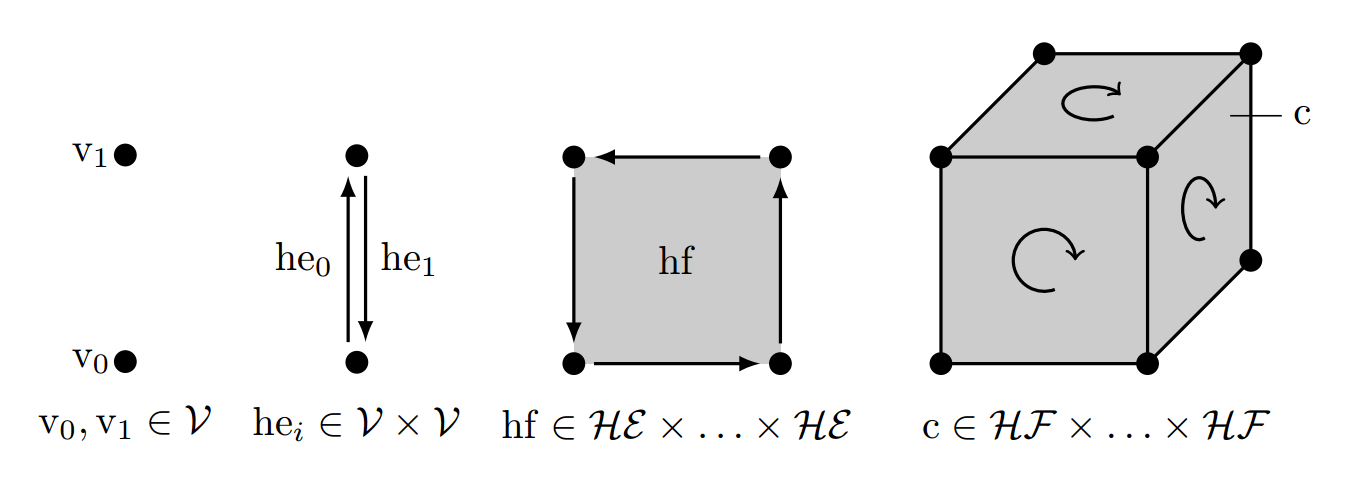
\includegraphics[width=.7\textwidth]{half-face_top_down.png}
    \caption[half-face从上到下的关系]{从上到下的关系信息示意图,对于除顶点外任意一层的元素,都包含一个用来构成它的下一层元素的一个有序列表,这些下层元素的排列顺序,决定了这个上层元素的朝向。图来自\cite{open-volume-mesh}}
    \label{fig:half-face-top-down}
\end{figure}

\begin{figure}[htbp]
    \centering
    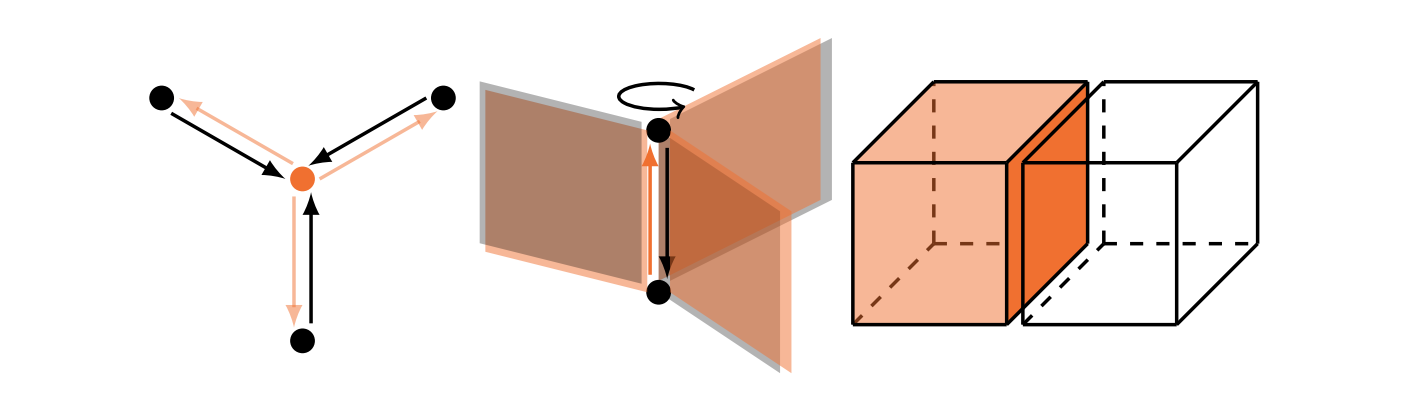
\includegraphics[width=.7\textwidth]{half-face_down_top.png}
    \caption[half-face从下到上的关系]{从下到上的关系信息示意图,对于除多面体外的任意一层的元素,都包含一个需要用它来构成的更上一层的元素的有序列表。图来自\cite{open-volume-mesh}}
    \label{fig:half-face-down-top}
\end{figure}
从上面half-face多面体网格的数据结构的描述中,我们可以看到,邻接信息的存储非常到位,对于任意一层的元素通过很少的查询,就能找到与其相邻的任意一层的元素列表,也就是说在half-face这个数据结构上信息的查询操作非常高效(比如查询一个顶点的邻接点,查询一个面的邻接多面体等等)。然而对于消边操作,由于需要维护很多的邻接关系,不仅复杂而且非常低效。\par
幸运的是,CGAL不仅给我们提供了鲁棒可靠的3D Delaunay三角化算法,而且给我们提供了一种很号的四面体网格数据结构Triangulation\_3d,其能够非常好地满足我们的需求——简单高效。在 CGAL的四面体数据结构中,包含两种最基本的数据:顶点和四面体,而边和面则通过四面体和顶点的组合来表示。对于每一个四面体,存储了该四面体的四个顶点的handle和分别与其四个面相邻接的四个四面体的handle;对于每一个顶点,存储了包含该顶点的某一个四面体的handle。通过这个简单的拓扑关系,我们就能够较为高效地查询出该四面体网格上的邻接信息,而且在做消边时也能够较为高效地维护该数据结构。

\section{密度为$\sigma$的均匀采样}
对于三角形上密度为$\sigma$的均匀采样,一种简单的均匀采样方法是为三角形做一个从全局到局部的坐标变换,使得一条边在x或y轴上,然后在其包围矩形上均匀采样,并选取属于这个三角形内的采样点(如图\ref{fig:direct-sampling-0})。但是这种方法并不鲁棒,对于有些三角形,该方法无法保证密度为$\sigma$这个条件——即以每个采样点为圆心,以$\sigma$为半径的圆能将这个三角形全部覆盖(如图\ref{fig:direct-sampling-1})。为此,我们想出了一种更好地采样方法:我们知道对于$\triangle ABC$中的任意一个采样点s都可以表示为(如图\ref{fig:param-sampling-convert}):
\begin{equation}
  \begin{split}
    s = \lambda_0 \overrightarrow{AC}+\lambda_1 \overrightarrow{AB} + A\\
    \lambda_0 + \lambda_1 \leq 1, \quad \lambda_0 \geq 0, \quad \lambda_1 \geq 0
  \end{split}
\end{equation}
因此,我们可以通过对$\lambda_0$和$\lambda_1$分别做密度为$\frac{\sigma}{\parallel \overrightarrow{AC} \parallel}$和$\frac{\sigma}{\parallel \overrightarrow{AB} \parallel}$的采样,从而间接得到$(\lambda_0,\lambda_1)$的采样,从而间接计算得到$\triangle ABC$上密度为$\sigma$的均匀采样。该采样算法能鲁棒地得到密度为$\sigma$的均匀采样(如图\ref{fig:param-sampling-0})。也可以采用相同的思想在四面体内做密度为$\sigma$的均匀采样,这里不再赘述。然而这种算法也还不够完美,采样点在三角形的边界处明显过密(如图\ref{fig:param-sampling-1})。为此,在这里使用一种基于网格细分的采样方法——对于给定的采样密度$\sigma$,我们不断遍历输入网格的每一条边,若其边长大于$\delta(\sigma)$,则我们对这条边做一个平均细分,直到所有的边的边长均小于$\delta(\sigma)$。最后我们将细分之后的三角网格上的顶点作为采样点。当$\delta(\sigma)=2\sigma/\sqrt{3}$即每一个三角形的每条边长都小于$2\sigma/\sqrt{3}$时,每一个三角形的外接圆半径小于$\sigma$,从而任一一个三角形的三个顶点上半径为$\sigma$的圆能将该三角形覆盖,从而满足采样密度要求。证明如下:设任一三角形上的最大边e的长为$x$,最大边对应的外接圆圆心角为$\alpha = 2\theta$(如图\ref{fig:max-len-calc}),则我们有
\begin{equation}
  \frac{x}{2r} = sin\theta, \theta \in [\pi/3, \pi/2] \qquad
  \Rightarrow \qquad r =\frac{x}{2} * \frac{1}{sin \theta} \leq \frac{x}{2} * \sqrt{3}
\end{equation}

\begin{figure}[htbp]
  \centering
  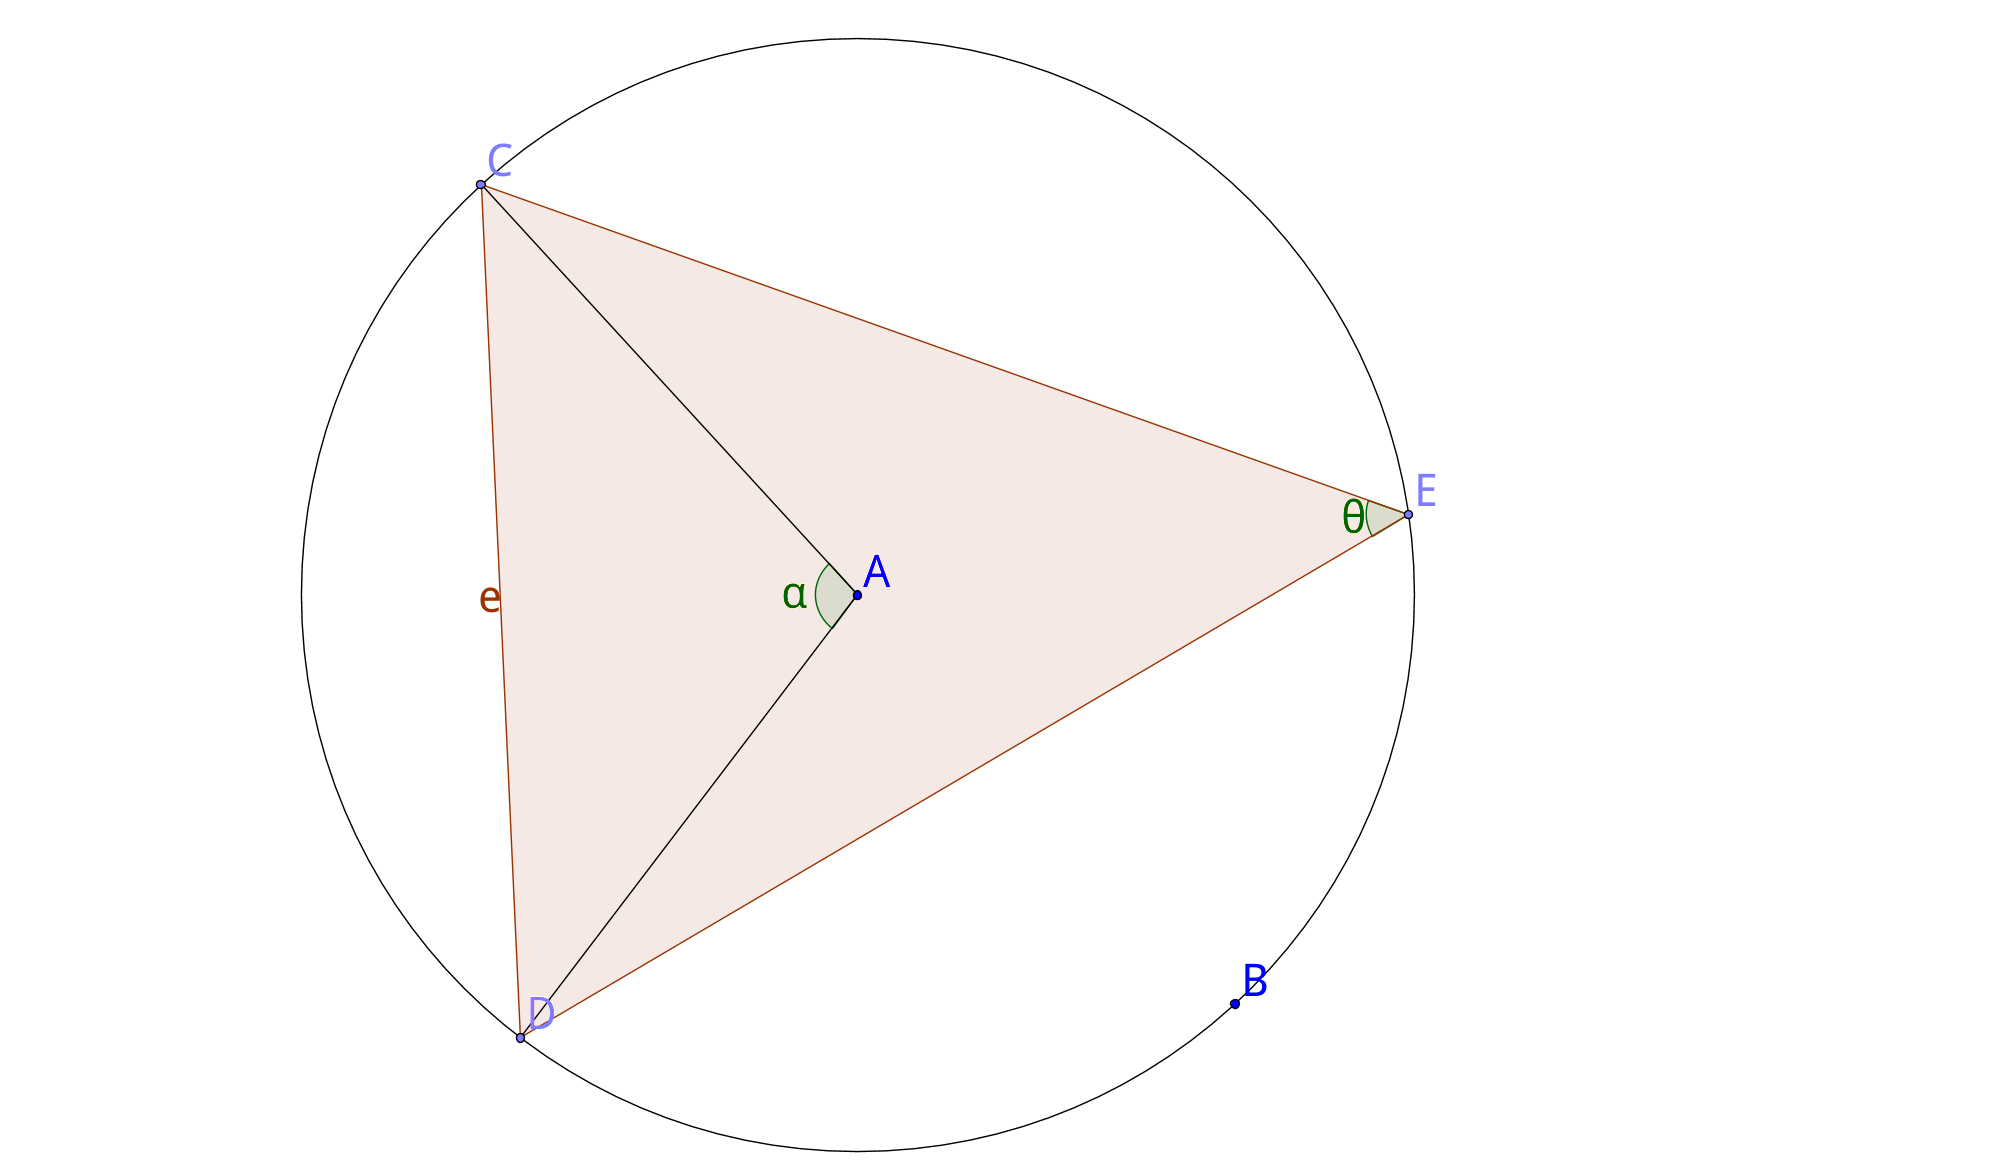
\includegraphics[width=0.8\textwidth]{max_len_calc.png}
  \caption[均匀采样细分阈值]{均匀采样时,是否需要继续细分阈值的计算示意图。}
  \label{fig:max-len-calc}
\end{figure}

\begin{figure}[htbp]
  \centering
  \begin{subfigure}[b]{0.4\textwidth}
    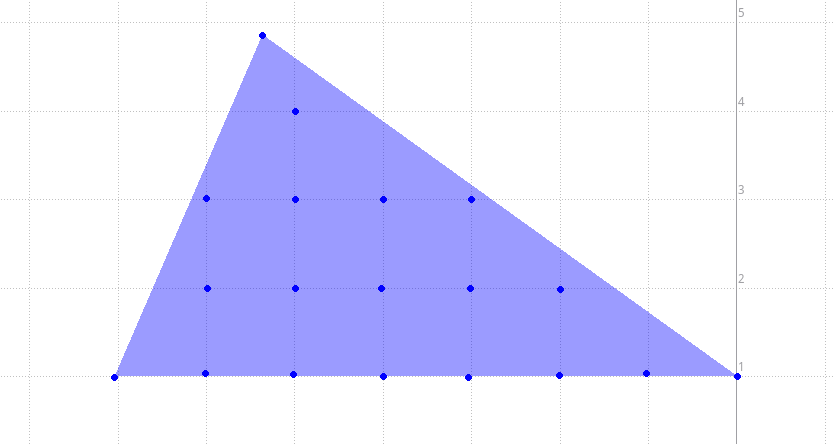
\includegraphics[width=\textwidth]{sampling_tris_basic.png}
    \caption{最直接的均匀采样方法,通过均匀撒点,然后选取在这个三角形内部的顶点作为采样结果。}
    \label{fig:direct-sampling-0}
  \end{subfigure}
  \begin{subfigure}[b]{0.8\textwidth}
      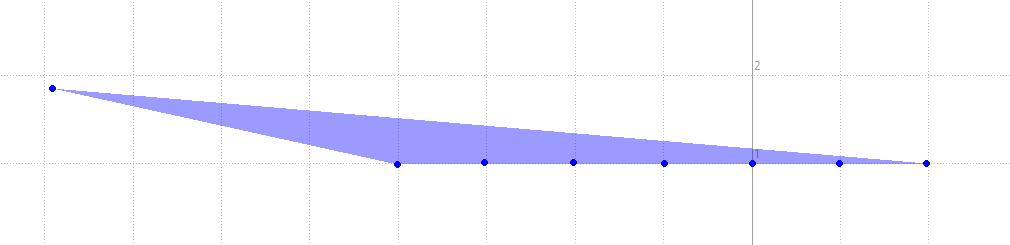
\includegraphics[width=\textwidth]{sampling_tris_fail.png}
      \caption{最直接的均匀采样方法无法保证以每一个采样点为圆心$\sigma$为半径的圆能够将整个三角形覆盖。该三角形左上方区域缺少采样点。}
    \label{fig:direct-sampling-1}
  \end{subfigure}
  \caption[最直接的采样及其问题]{最直接的均匀采样的示意图}
  \label{fig:direct-sampling}
\end{figure}

\begin{figure}[htbp]
  \centering
  \begin{subfigure}[b]{0.8\textwidth}
    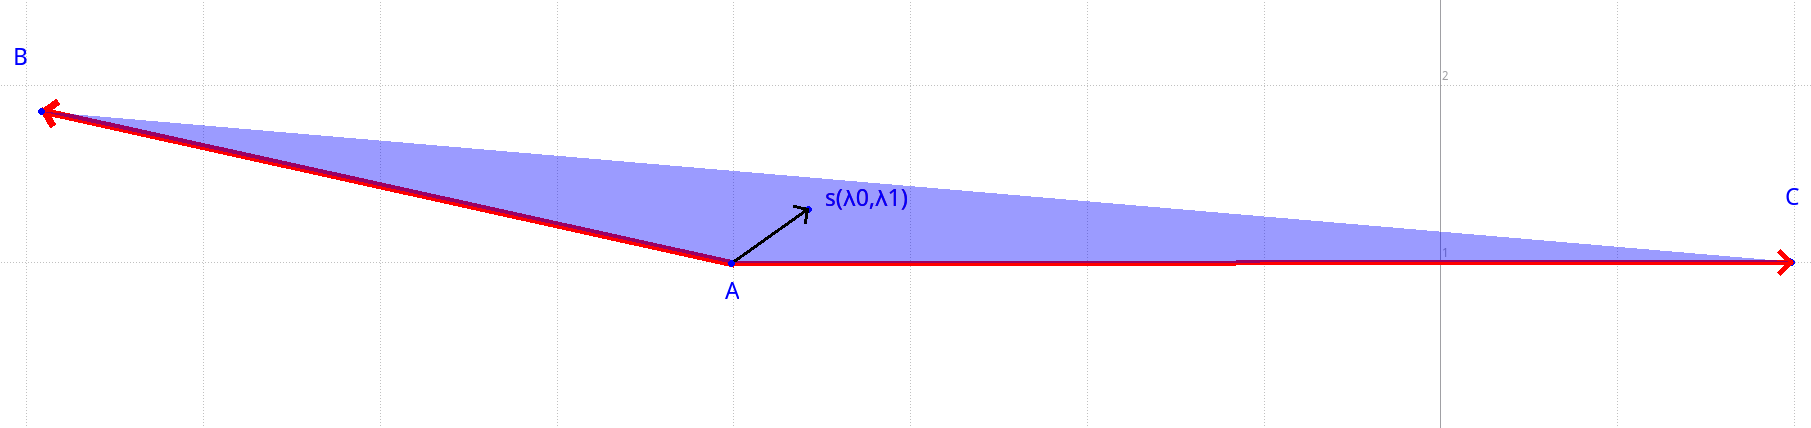
\includegraphics[width=\textwidth]{sample_tris_convert.png}
    \caption{通过对$\lambda_0$,$\lambda_1$的采样来得到该三角形的密度为$\sigma$的均匀采样。}
    \label{fig:param-sampling-convert}
  \end{subfigure}
  \begin{subfigure}[b]{0.8\textwidth}
      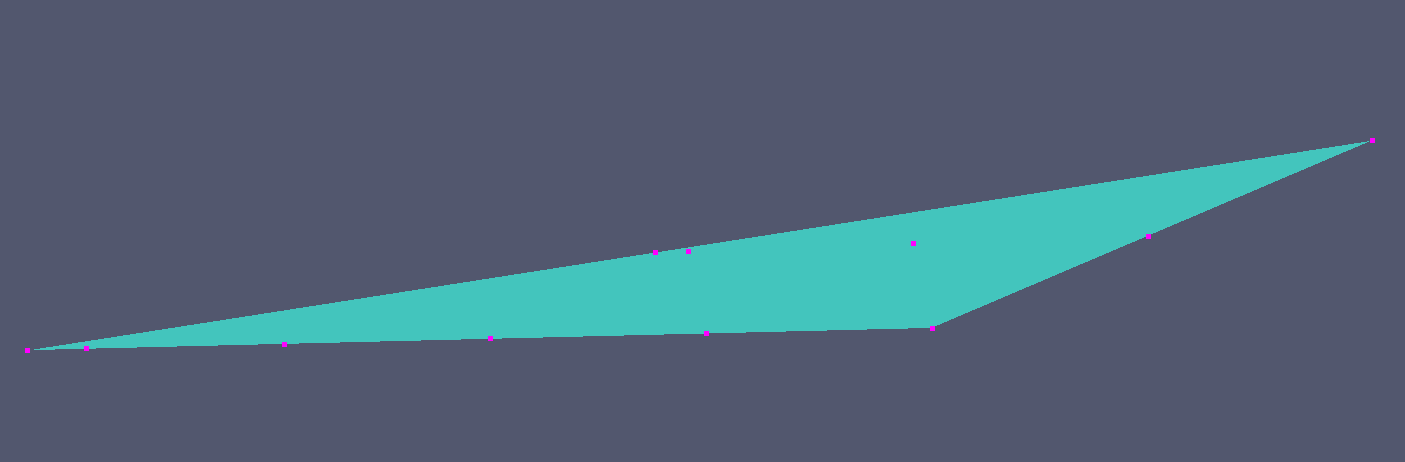
\includegraphics[width=\textwidth]{param_sampling_0.png}
      \caption{该均匀采样算法能够鲁棒地处理细长三角形,保证每一个采样点为圆心$\sigma$为半径的圆能够将整个三角形覆盖。}
      \label{fig:param-sampling-0}
  \end{subfigure}
  \begin{subfigure}[b]{0.8\textwidth}
      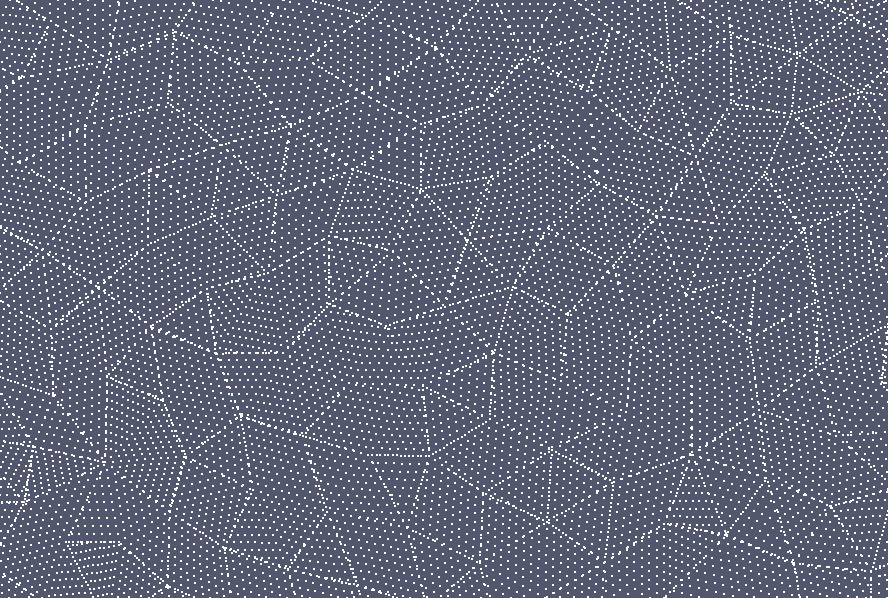
\includegraphics[width=\textwidth]{param_sampling_1.png}
      \caption{该方法的到的采样的结果,采样点在三角形的边界处明显过密。}
      \label{fig:param-sampling-1}
  \end{subfigure}
  \caption[转换参数的采样方法]{转换采样参数的均匀采样方法}
  \label{fig:param-sampling}
\end{figure}

\section{Link Condition 和 Kernel Region 的检测}
对于是否满足Link Condition,我们通过查询包含顶点A的所有四面体中,不包含顶点A的边,得到边的集合e(A),同理得到e(B),再通过查询同时包含顶点AB的四面体中,不包含顶点A和B的边得到边的集合e(AB),从而Link Condition是否满足等价于$e(A) \cap e(B) = e(AB)$是否成立。 \par
对于AB的候选合并点是否落在其Kernel Region中,即AB的一环邻域的边界的每一个三角形内侧(如图\ref{fig:kr})。邻域边界上的三角面片,即为只包含顶点A或顶点B的四面体中,除了A和B之外的另外的三个顶点所构成的三角面片。通过查询邻接信息,我们可以得到只包含顶点A或B的两个四面体集合$tet(A),tet(B)$。我们将所有这些三角面片上的一个顶点$v_i$的及其法向$n_i$(指向内侧)保存下来,然后对于每个候选合并点$v_m$判断$(v_m − v_i) \cdot n_i > 0$,即可判断其是否落在Kernel Region中。
\begin{figure}[htbp]
    \centering
    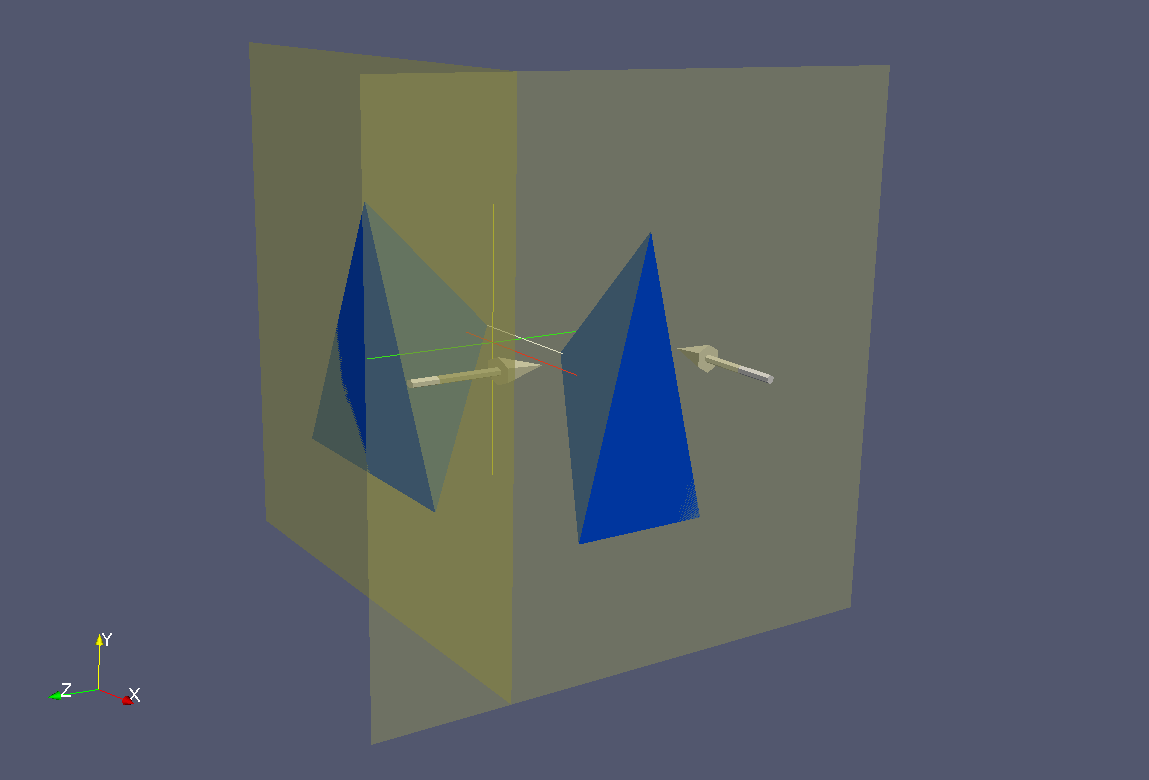
\includegraphics[width=.7\textwidth]{kr.png}
    \caption[3D Kernel Region]{对于一条边AB其Kernel Region是其一环邻域的边界上的每个三角形的内侧。图中显示了一条白色的边,以及其一环邻域中的两个四面体以及其对应的有向平面(黄色以及指向内侧的箭头),其Kernel Region是这些有向平面的内侧的交集。}
    \label{fig:kr}
\end{figure}

\section{误差判断条件的检测}
对于每一个消边后新生成的四面体$tet(v_0, v_1, v_2, v_3)$,每个采样点在这个四面体上都有唯一的重心坐标$(w_0, w_1, w_2, w_3)$。我们可以通过求解如下线性方程组来得到采样点s的重心坐标:$[v_0, v_1, v_2, v_3] \cdot [w_0, w_1, w_2, w_3]^T=s$,并根据重心坐标来判断顶点是否落在这个四面体内部——$\forall w_i>0, \sum_{i=0}^3 w_i \leq 1$,若采样点落在四面体内部,则可以可通过线性差值\eqref{eq:linear-interpolation},计算出该采样点的$\epsilon(s)$,从而判断采样点是否满足误差约束条件。

\section{消边操作}
消边操作是最基础也是重要的数据操作。在消边操作中涉及到的是操作有顶点的删除与添加、边的删除与添加、四面体的删除与添加。我们采用一种生成洞并补洞的消边方法,首先将所有包含AB的四面体从四面体网格$\tau$中移除,生成一个洞。然后再加入合并点,与该洞的边界上的面构成新的四面体,然后再更新洞的边界的四面体的邻接信息。
